\documentclass[letter,10pt]{article}

\usepackage[spanish,es-nodecimaldot]{babel}
\usepackage[utf8]{inputenc}

\renewcommand{\familydefault}{\sfdefault}
\usepackage[T1]{fontenc}
\usepackage{textcomp}

\usepackage{framed}
\usepackage[svgnames]{xcolor}
\colorlet{shadecolor}{Gainsboro!50}

\usepackage{enumitem}
\usepackage{graphicx}
\usepackage{pstricks}

\usepackage{anysize}
\marginsize{3cm}{2cm}{2cm}{3cm}

\usepackage{float}
\usepackage{siunitx}
\usepackage{amsmath}
\usepackage{array}

\usepackage{multicol}
\usepackage{pifont}

\usepackage{fancyhdr}
\usepackage{lastpage}
\pagestyle{fancy}
\fancyhf{}
\fancyhead[LE,RO]{Termodinámica}
\fancyfoot[CO,CE]{\thepage\ de \pageref{LastPage}}

\special{papersize=215.9mm,279.4mm}

\usepackage[
    pdfauthor={Carlos Eduardo Caballero Burgoa},%
    pdftitle={Termodinámica},%
    pdfsubject={Practica 05},%
    colorlinks,%
    citecolor=black,%
    filecolor=black,%
    linkcolor=black,%
    urlcolor=black,
    breaklinks]{hyperref}
\usepackage{breakurl}

\renewcommand{\arraystretch}{1.2}

\begin{document}

\begin{center}
    {\Large \bf{Practica \#05}}
\end{center}
\vspace{0.20cm}

\begin{enumerate}

\item A una turbina de vapor ingresan 2 flujos de agua con baja velocidad. Vapor
con alta presión entra por el punto (1) a $2[\text{MPa}]$, $500^\circ\text{C}$ y
$2[\text{kg}/\text{s}]$. Por el punto (2) entra agua de enfriamiento a
$120[\text{kPa}]$, $30^\circ\text{C}$ y $0.3[\text{kg}/\text{s}]$. La mezcla
sale por (3) a $150[\text{kPa}]$, $80\%$ de titulo, a través de un ducto de
$0.15[\text{m}]$ de diámetro. Se tiene una perdida de calor de $300[\text{kW}]$.
Hallar la velocidad de salida y la potencia generada por la maquina.

\begin{figure}[H]
\centering
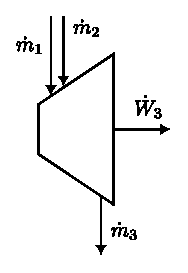
\includegraphics[scale=1.0]{resources/f01.eps}
\end{figure}

\textbf{\underline{Solución}:} \\

\begin{center}
\begin{tabular}{l l l|l}
\ding{172} Agua     & \ding{173} Agua       & \ding{174} Agua & \text{Turbina}      \tabularnewline \hline
$P_1=2000[kPa]$     & $P_2=120[kPa]$        & $P_3=150[kPa]$  & $\dot{Q}_3=300[kW]$ \tabularnewline
$T_1=500^\circ C$   & $T_2=30^\circ C$      & $X_3=0.8$       & $\dot{W}_3=?$       \tabularnewline
$\dot{m}_1=2[kg/s]$ & $\dot{m}_2=0.3[kg/s]$ & $d_3=0.15[m]$   &                     \tabularnewline
$v_1 \approx 0$     & $v_2 \approx 0$       & $v_3=?$         &                     \tabularnewline
\end{tabular}
\end{center}

Se plantean las ecuaciones de equilibrio:

\begin{equation*}
    \sum\dot{Q} + \sum\dot{m}_E (h_E + \frac{v^2_E}{2} + g z_E) =
    \sum\dot{W} + \sum\dot{m}_S (h_S + \frac{v^2_S}{2} + g z_S)
\end{equation*}
\begin{equation*}
    \sum\dot{Q} + \sum\dot{m}_E (h_E + 0 + 0) =
    \sum\dot{W} + \sum\dot{m}_S (h_S + \frac{v^2_S}{2} + 0)
\end{equation*}

Por tanto:

\begin{eqnarray*}
    -\dot{Q}_3 + \dot{m}_1 h_1 + \dot{m}_2 h_2
    = \dot{W}_3 + \dot{m}_3 h_3 + \frac{v^2_3}{2} \\
    \dot{m}_1 + \dot{m}_2 = \dot{m}_3 \\
    \dot{m}_3 = A\,\frac{v_3}{\nu_3} = \pi\frac{d^2_3}{4}\frac{v_3}{\nu_3}
\end{eqnarray*}

\ding{172}
\begin{eqnarray*}
    \begin{array}{c}
        P_1 = 2000[kPa] \\
        T_1 = 500^\circ C
    \end{array}
    \rightarrow
    \begin{cases}
        X_1 > 1 \\
        h_1 = 3467.55[kJ/kg]
    \end{cases}
\end{eqnarray*}

\ding{173}
\begin{eqnarray*}
    \begin{array}{c}
        P_2 = 120[kPa] \\
        T_2 = 30^\circ C
    \end{array}
    \rightarrow
    \begin{cases}
        X_2 = 0 \\
        h_2 = 125.77[kJ/kg]
    \end{cases}
\end{eqnarray*}

\ding{174}
\begin{eqnarray*}
    \begin{array}{c}
        P_3 = 150[kPa] \\
        X_3 = 0.8
    \end{array}
    \rightarrow
    \begin{cases}
        T_3 = 111.37^\circ C \\
        \nu_l = 0.001053[m^3/kg] \\
        \nu_v = 1.15933[m^3/kg] \\
        \nu_3 = \nu_l + X_3 (\nu_v - \nu_l) = 0.9277[m^3/kg] \\
        h_l = 467.08[kJ/kg] \\
        h_v = 2693.54[kJ/kg] \\
        h_3 = h_l + X_3 (h_v - h_l) = 2248.2[kJ/kg]
    \end{cases}
\end{eqnarray*}

\begin{figure}[H]
\centering
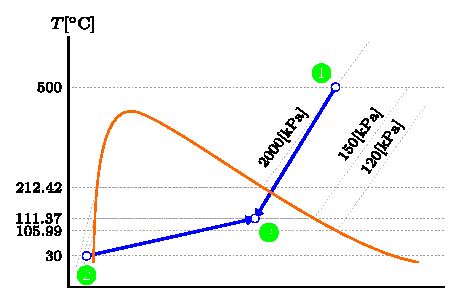
\includegraphics[scale=1.25]{resources/g01.eps}
\end{figure}

Se calcula $\dot{m}_3$:

\begin{eqnarray*}
    \dot{m}_3 &=& \dot{m}_1 + \dot{m}_2 \\
              &=& 2[kg/s] + 0.3[kg/s] \\
              &=& 2.3[kg/s]
\end{eqnarray*}

Se calcula $v_3$:

\begin{eqnarray*}
    v_3 &=& \dot{m}_3\frac{4\,\nu_3}{\pi\,d^2_3} \\
         &=& 2.3[kg/s]\frac{4(0.9277[m^3/kg])}{\pi(0.15^2[m^2])} \\
         &=& 120.74[m/s]
\end{eqnarray*}

\begin{equation*}
\boxed{
    \begin{array}{l}
        v_3 = 120.74[\text{m}/\text{s}]
    \end{array}
}
\end{equation*}

Se calcula $\dot{W}_3$:

\begin{eqnarray*}
    \dot{W}_3 &=& \dot{m}_1 h_1 + \dot{m}_2 h_2 - \dot{m}_3 h_3
                - \dot{m}_3\frac{v^2_3}{2} - \dot{Q}_3 \\
              &=& 2[kg/s] 3467.55[kJ/kg] + 0.3[kg/s] 125.77[kJ/kg]
                - 2.3[kg/s] 2248.2[kJ/kg] \\
              &-& 0.5 (2.3[kg/s]) (120.74)^2[m^2/s^2] - 300[kW] \\
              &=& 1500.9[kW]
\end{eqnarray*}

\begin{equation*}
\boxed{
    \begin{array}{l}
        \dot{W}_3 = 1500.9[\text{kW}]
    \end{array}
}
\end{equation*}

\noindent\rule{15.2cm}{0.4pt}

\item A un intercambiador de calor ingresan los humos de combustión para
pre-calentar el agua. Los humos entran a $500^\circ\text{C}$,
$101.3[\text{kPa}]$ y salen a $150^\circ\text{C}$. El agua entra a
$100^\circ\text{C}$ y $1[\text{MPa}]$ y sale como vapor saturado a
$1[\text{MPa}]$. Los humos tienen calor especifico
$C_p = 1.05[\text{kJ}/\text{kg}\,\text{K}]$ y pueden ser tratados como aire (
$h = C_p\,T$). Si el flujo de los humos es de $25000[\text{kg}/\text{h}]$,
hallar el flujo de agua que se puede calentar en ese intercambiador.

\begin{figure}[H]
\centering
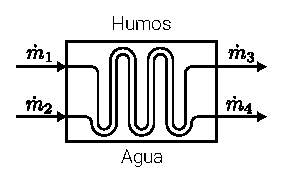
\includegraphics[scale=1.0]{resources/f02.eps}
\end{figure}

\textbf{\underline{Solución}:} \\

\begin{center}
\begin{tabular}{l l l l}
\ding{172} Humo         & \ding{173} Agua   & \ding{174} Humo   & \ding{175} Agua \tabularnewline \hline
$T_1=500^\circ C$       & $T_2=100^\circ C$ & $T_3=150^\circ C$ & $X_4=1$         \tabularnewline
$P_1=101.3[kPa]$        & $P_2=1000[kPa]$   &                   & $P_4=1000[kPa]$ \tabularnewline
$\dot{m}_1=25000[kg/h]$ & $\dot{m}_2=?$     &                   &                 \tabularnewline
\end{tabular}
\end{center}

La capacidad calorífica del humo es: $C_p = 1.05[kJ/kg\,K]$.

La entalpía para el humo se calculará a partir de la ecuación: $h = C_p\,T$.

Se plantean las ecuaciones de equilibrio:

\begin{equation*}
    \sum\dot{Q} + \sum\dot{m}_E (h_E + \frac{v^2_E}{2} + g z_E) =
    \sum\dot{W} + \sum\dot{m}_S (h_S + \frac{v^2_S}{2} + g z_S)
\end{equation*}
\begin{equation*}
    0 + \sum\dot{m}_E (h_E + 0 + 0) = 0 + \sum\dot{m}_S (h_S + 0 + 0)
\end{equation*}

Por tanto:

\begin{eqnarray*}
    \dot{m}_1 h_1 + \dot{m}_2 h_2 = \dot{m}_3 h_3 + \dot{m}_4 h_4 \\
    \dot{m}_1 = \dot{m}_3 \\
    \dot{m}_2 = \dot{m}_4
\end{eqnarray*}

\ding{172}
\begin{equation*}
    h_1 = C_p\,T_1 = 1.05[kJ/kg\,K] (500 + 273.15)[K] = 811.81[kJ/kg]
\end{equation*}

\ding{174}
\begin{equation*}
    h_3 = C_p\,T_1 = 1.05[kJ/kg\,K] (150 + 273.15)[K] = 444.31[kJ/kg]
\end{equation*}

\ding{173}
\begin{eqnarray*}
    \begin{array}{c}
        T_2 = 100^\circ C \\
        P_2 = 1000[kPa]
    \end{array}
    \rightarrow
    \begin{cases}
        X_2 = 0 \\
        h_2 = 419.02[kJ/kg]
    \end{cases}
\end{eqnarray*}

\ding{175}
\begin{eqnarray*}
    \begin{array}{c}
        X_4 = 1 \\
        P_4 = 1000[kPa]
    \end{array}
    \rightarrow
    \begin{cases}
        T_4 = 179.91^\circ C \\
        h_4 = 2778.08[kJ/kg]
    \end{cases}
\end{eqnarray*}

\begin{figure}[H]
\centering
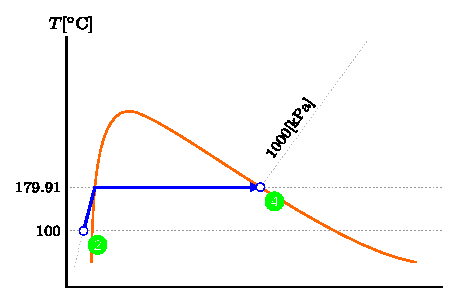
\includegraphics[scale=1.25]{resources/g02.eps}
\end{figure}

Se calcula $\dot{m}_2$:

\begin{eqnarray*}
    \dot{m}_1 h_1 + \dot{m}_2 h_2 = \dot{m}_3 h_3 + \dot{m}_4 h_4 \\
    \dot{m}_1 h_1 + \dot{m}_2 h_2 = \dot{m}_1 h_3 + \dot{m}_2 h_4 \\
    \dot{m}_2 (h_2 - h_4) = \dot{m}_1 (h_3 - h_1) \\
\end{eqnarray*}
\begin{eqnarray*}
    \dot{m}_2 &=& \dot{m}_1\frac{h_3 - h_1}{h_2 - h_4} \\
              &=& 25000[kg/h]\left(
                  \frac{444.31[kJ/kg]-811.81[kJ/kg]}
                  {419.02[kJ/kj]-2778.08[kJ/kg]}
                  \right) \\
              &=& 3894.6[kg/h]
\end{eqnarray*}

\begin{equation*}
\boxed{
    \begin{array}{l}
        \dot{m}_2 = 3894.6[\text{kg}/\text{h}]
    \end{array}
}
\end{equation*}

\noindent\rule{15.2cm}{0.4pt}

\item En el evaporador de un equipo de frío se enfría aire atmosférico desde
$18^\circ\text{C}$ a $-5^\circ\text{C}$. El freón 12 que pasa por el evaporador
entra a $-10^\circ\text{C}$ y titulo de $35\%$ y sale como vapor saturado a
$-10^\circ\text{C}$. Si por las paredes del intercambiador ingresa a
$400[\text{kJ}/\text{min}]$ de flujo de calor. Hallar para un flujo de aire de
$150[\text{kg}/\text{s}]$ de aire el caudal másico de freón 12.

\begin{figure}[H]
\centering
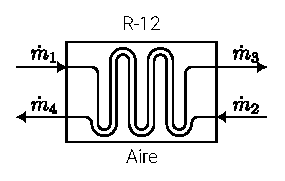
\includegraphics[scale=1.0]{resources/f03.eps}
\end{figure}

\textbf{\underline{Solución}:} \\

\begin{center}
\begin{tabular}{l l l l|l}
\ding{172} Aire       & \ding{173} R-12   & \ding{174} Aire  & \ding{175} R-12   & Intercambiador        \tabularnewline \hline
$T_1=18^\circ C$      & $T_2=-10^\circ C$ & $T_3=-5^\circ C$ & $T_4=-10^\circ C$ & $\dot{Q}=400[kJ/min]$ \tabularnewline
$\dot{m}_1=150[kg/s]$ & $X_2=0.35$        &                  & $X_4=1$           &                       \tabularnewline
\end{tabular}
\end{center}

La capacidad calorífica del aire es: $C_p = 1.005[kJ/kg\,K]$.

La entalpía para el aire se calculará a partir de la ecuación: $h = C_p\,T$.

Se plantean las ecuaciones de equilibrio:

\begin{equation*}
    \sum\dot{Q} + \sum\dot{m}_E (h_E + \frac{v^2_E}{2} + g z_E) =
    \sum\dot{W} + \sum\dot{m}_S (h_S + \frac{v^2_S}{2} + g z_S)
\end{equation*}
\begin{equation*}
    \sum\dot{Q} + \sum\dot{m}_E (h_E + 0 + 0) = 0 + \sum\dot{m}_S (h_S + 0 + 0)
\end{equation*}

Por tanto:

\begin{eqnarray*}
    \dot{Q} + \dot{m}_1 h_1 + \dot{m}_2 h_2 = \dot{m}_3 h_3 + \dot{m}_4 h_4 \\
    \dot{m}_1 = \dot{m}_3 \\
    \dot{m}_2 = \dot{m}_4
\end{eqnarray*}

\ding{172}
\begin{equation*}
    h_1 = C_p\,T_1 = 1.005[kJ/kg\,K] (18 + 273.15)[K] = 292.61[kJ/kg]
\end{equation*}

\ding{174}
\begin{equation*}
    h_3 = C_p\,T_1 = 1.005[kJ/kg\,K] (-5 + 273.15)[K] = 269.49[kJ/kg]
\end{equation*}

\ding{173}
\begin{eqnarray*}
    \begin{array}{c}
        T_2 = -10^\circ C \\
        X_2 = 0.35
    \end{array}
    \rightarrow
    \begin{cases}
        h_l = 26.874[kJ/kg] \\
        h_v = 183.188[kJ/kg] \\
        h_2 = h_l + X_2 (h_v - h_l) = 81.584[kJ/kg]
    \end{cases}
\end{eqnarray*}

\ding{175}
\begin{eqnarray*}
    \begin{array}{c}
        T_4 = -10^\circ C \\
        X_4 = 1
    \end{array}
    \rightarrow
    \begin{cases}
        h_4 = 183.188[kJ/kg]
    \end{cases}
\end{eqnarray*}

\begin{figure}[H]
\centering
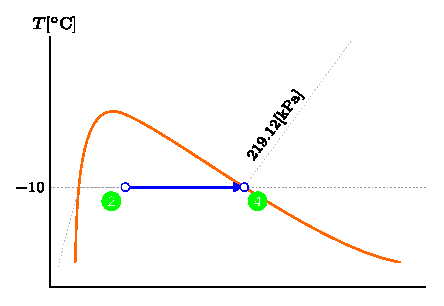
\includegraphics[scale=1.25]{resources/g03.eps}
\end{figure}

Se calcula $\dot{m}_2$:

\begin{eqnarray*}
    \dot{Q} + \dot{m}_1 h_1 + \dot{m}_2 h_2 = \dot{m}_3 h_3 + \dot{m}_4 h_4 \\
    \dot{Q} + \dot{m}_1 h_1 + \dot{m}_2 h_2 = \dot{m}_1 h_3 + \dot{m}_2 h_4 \\
    \dot{m}_2 (h_2 - h_4) = \dot{m}_1 (h_3 - h_1) - \dot{Q} \\
\end{eqnarray*}
\begin{eqnarray*}
    \dot{m}_2 &=& \frac{\dot{m}_1 (h_3 - h_1) - \dot{Q}}{h_2 - h_4} \\
              &=& \frac{150 [\frac{kg}{s}]\left(269.49[\frac{kJ}{kg}]
              - 292.61[\frac{kJ}{kg}]\right)
              - 400[\frac{kJ}{min}]\frac{1[min]}{60[s]}}{81.584[kJ/kg]
              - 183.188[kJ/kg]} \\
              &=& 34.191[kg/s]
\end{eqnarray*}

\begin{equation*}
\boxed{
    \begin{array}{l}
        \dot{m}_2 = 34.191[\text{kg}/\text{s}]
    \end{array}
}
\end{equation*}

\noindent\rule{15.2cm}{0.4pt}

\item Según la figura, refrigerante 12 a $1[\text{MPa}]$ y $80^\circ\text{C}$ es
enfriado a $1[\text{MPa}]$ y $30^\circ\text{C}$ en un condensador con aire
atmosférico que entra con $100[\text{kPa}]$ y $27^\circ\text{C}$ y sale con
$60^\circ\text{C}$. Hallar el flujo másico de refrigerante para un flujo de aire
de $2[kg/s]$.

\begin{figure}[H]
\centering
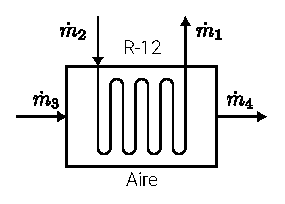
\includegraphics[scale=1.0]{resources/f04.eps}
\end{figure}

\textbf{\underline{Solución}:} \\

\begin{center}
\begin{tabular}{l l l l}
\ding{172} R-12  & \ding{173} R-12  & \ding{174} Aire     & \ding{175} Aire  \tabularnewline \hline
$P_1=1000[kPa]$  & $P_2=1000[kPa]$  & $P_3=100[kPa]$      & $P_4=100[kPa]$   \tabularnewline
$T_1=80^\circ C$ & $T_2=30^\circ C$ & $T_3=27^\circ C$    & $T_4=60^\circ C$ \tabularnewline
$\dot{m}_1=?$    &                  & $\dot{m}_3=2[kg/s]$ &                  \tabularnewline
\end{tabular}
\end{center}

La capacidad calorífica del aire es: $C_p = 1.005[kJ/kg\,K]$.

La entalpía para el aire se calculará a partir de la ecuación: $h = C_p\,T$.

Se plantean las ecuaciones de equilibrio:

\begin{equation*}
    \sum\dot{Q} + \sum\dot{m}_E (h_E + \frac{v^2_E}{2} + g z_E) =
    \sum\dot{W} + \sum\dot{m}_S (h_S + \frac{v^2_S}{2} + g z_S)
\end{equation*}
\begin{equation*}
    0 + \sum\dot{m}_E (h_E + 0 + 0) = 0 + \sum\dot{m}_S (h_S + 0 + 0)
\end{equation*}

Por tanto:

\begin{eqnarray*}
    \dot{m}_1 h_1 + \dot{m}_3 h_3 = \dot{m}_2 h_2 + \dot{m}_4 h_4 \\
    \dot{m}_1 = \dot{m}_2 \\
    \dot{m}_3 = \dot{m}_4
\end{eqnarray*}

\ding{172}
\begin{eqnarray*}
    \begin{array}{c}
        P_1 = 1000[kPa] \\
        T_1 = 80^\circ C
    \end{array}
    \rightarrow
    \begin{cases}
        X_1 > 1 \\
        h_1 = 232.910[kJ/kg]
    \end{cases}
\end{eqnarray*}

\ding{173}
\begin{eqnarray*}
    \begin{array}{c}
        P_2 = 1000[kPa] \\
        T_2 = 30^\circ C
    \end{array}
    \rightarrow
    \begin{cases}
        X_2 = 0 \\
        h_2 = 64.592[kJ/kg]
    \end{cases}
\end{eqnarray*}

\ding{174}
\begin{equation*}
    h_3 = C_p\,T_3 = 1.005[kJ/kg\,K] (27 + 273.15)[K] = 301.65[kJ/kg]
\end{equation*}

\ding{175}
\begin{equation*}
    h_4 = C_p\,T_4 = 1.005[kJ/kg\,K] (60 + 273.15)[K] = 334.82[kJ/kg]
\end{equation*}

\begin{figure}[H]
\centering
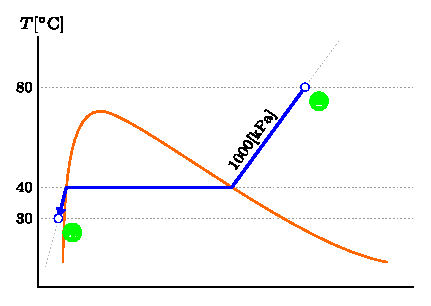
\includegraphics[scale=1.25]{resources/g04.eps}
\end{figure}

Se calcula $\dot{m}_1$:

\begin{eqnarray*}
    \dot{m}_1 h_1 + \dot{m}_3 h_3 = \dot{m}_2 h_2 + \dot{m}_4 h_4 \\
    \dot{m}_1 h_1 + \dot{m}_3 h_3 = \dot{m}_1 h_2 + \dot{m}_3 h_4 \\
    \dot{m}_1 (h_1 - h_2) = \dot{m}_3 (h_4 - h_3) \\
\end{eqnarray*}
\begin{eqnarray*}
    \dot{m}_1 &=& \dot{m}_3\frac{h_4 - h_3}{h_1 - h_2} \\
              &=& 2[kg/s]\left(\frac{334.82[kJ/kg]-301.65[kJ/kg]}{232.910[kJ/kj]
                - 64.592[kJ/kg]}\right) \\
              &=& 0.3941[kg/s]
\end{eqnarray*}

\begin{equation*}
\boxed{
    \begin{array}{l}
        \dot{m}_1 = 0.3941[\text{kg}/\text{s}]
    \end{array}
}
\end{equation*}

\noindent\rule{15.2cm}{0.4pt}

\item Se tiene un mezclador de agua liquida y vapor saturado según figura, por
un ducto (2) ingresa $7513[\text{kg}/\text{h}]$ de vapor con
$165[\text{m}/\text{min}]$, $1.5[\text{MPa}]$. Por el otro ducto (1)
ingresa $1150[\text{kg}/\text{h}]$ de agua a $980[\text{kPa}]$ y $80^\circ C$.
Ambos fluidos se mezclan antes del ducto de salida el cual tiene un área de
$0.2[\text{m}^2]$, $0.275[\text{MPa}]$ de presión y $100[\text{m}/\text{min}]$
de velocidad. Por las paredes del mezclador se pierde calor a razón de
$2000[\text{kJ}/\text{h}]$. Se desea enfriar estos dos fluidos para lo cual se
usa freón 134a que ingresa a $200[\text{kPa}]$, $-20^\circ\text{C}$ y sale a
$300[\text{kPa}]$ y $50^\circ\text{C}$. Hallar el caudal másico de R134a que se
requiere.

\begin{figure}[H]
\centering
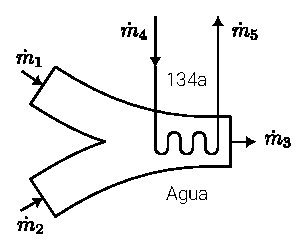
\includegraphics[scale=1.0]{resources/f05.eps}
\end{figure}

\textbf{\underline{Solución}:} \\

\begin{center}
\begin{tabular}{l l l l l}
\ding{172} Agua        & \ding{173} Agua        & \ding{174} Agua  & \ding{175} R134a  & \ding{176} R134a \tabularnewline \hline
$\dot{m}_1=1150[kg/h]$ & $\dot{m}_2=7513[kg/h]$ & $A_3=0.2[m^2]$   & $P_4=200[kPa]$    & $P_5=300[kPa]$   \tabularnewline
$P_1=980[kPa]$         & $v_2=165[m/min]$       & $P_3=275[kPa]$   & $T_4=-20^\circ C$ & $T_5=50^\circ C$ \tabularnewline
$T_1=80^\circ C$       & $P_2=1500[kPa]$        & $v_3=100[m/min]$ & $\dot{m}_4=?$     &                  \tabularnewline
$X_1=0$                & $X_2=1$                &                  &                   &                  \tabularnewline
\end{tabular}
\end{center}

Calor perdido: $\dot{Q} = 2000[kJ/h]$.

Se plantean las ecuaciones de equilibrio:

\begin{equation*}
    \sum\dot{Q} + \sum\dot{m}_E (h_E + \frac{v^2_E}{2} + g z_E) =
    \sum\dot{W} + \sum\dot{m}_S (h_S + \frac{v^2_S}{2} + g z_S)
\end{equation*}
\begin{equation*}
    \sum\dot{Q} + \sum\dot{m}_E (h_E + \frac{v^2_E}{2} + 0)
    = 0 + \sum\dot{m}_S (h_S + \frac{v^2_S}{2} + 0)
\end{equation*}

Por tanto:

\begin{eqnarray*}
    -\dot{Q} + \dot{m}_1 h_1 + \dot{m}_2 h_2 + \dot{m}_2 \frac{v^2_2}{2}
    + \dot{m}_4 h_4
    = \dot{m}_3 h_3 + \dot{m}_3 \frac{v^2_3}{2} + \dot{m}_5 h_5 \\
    \dot{m}_1 + \dot{m}_2 = \dot{m}_3 \\
    \dot{m}_4 = \dot{m}_5 \\
    \dot{m}_3 = A_3\,\frac{v_3}{\nu_3}
\end{eqnarray*}

\ding{172}
\begin{eqnarray*}
    \begin{array}{c}
        P_1 = 980[kPa] \\
        T_1 = 80^\circ C
    \end{array}
    \rightarrow
    \begin{cases}
        X_1 = 0 \\
        h_1 = 334.88[kJ/kg]
    \end{cases}
\end{eqnarray*}

\ding{173}
\begin{eqnarray*}
    \begin{array}{c}
        P_2 = 1500[kPa] \\
        X_2 = 1
    \end{array}
    \rightarrow
    \begin{cases}
        T_2 = 198.32^\circ C \\
        h_2 = 2792.15[kJ/kg]
    \end{cases}
\end{eqnarray*}

Se calcula $\dot{m}_3$:

\begin{eqnarray*}
    \dot{m}_3 &=& \dot{m}_1 + \dot{m}_2 \\
              &=& 1150[kg/h] + 7513[kg/h] \\
              &=& 8663[kg/h]
\end{eqnarray*}

Se calcula $\nu_3$:

\begin{eqnarray*}
    \nu_3 &=& A_3 \frac{v_3}{\dot{m}_3} \\
          &=& 0.2[m^2] \dfrac{100[\frac{m}{min}]\frac{60[min]}{1[h]}}
              {8663[\frac{kg}{h}]} \\
          &=& 0.1385[m^3/kg]
\end{eqnarray*}

\ding{174}
\begin{eqnarray*}
    \begin{array}{c}
        P_3 = 275[kPa] \\
        \nu_3 = 0.1385[m^3/kg]
    \end{array}
    \rightarrow
    \begin{cases}
        T_3 = 130.60^\circ C \\
        \nu_l = 0.001070[m^3/kg] \\
        \nu_v = 0.65731[m^3/kg] \\
        X_3 = \dfrac{\nu_3 - \nu_l}{\nu_v - \nu_l} = 0.2095 \\
        h_l = 548.87[kJ/kg] \\
        h_v = 2721.29[kJ/kg] \\
        h_3 = h_l + X_3 (h_v - h_l) = 1003.9[kJ/kg]
    \end{cases}
\end{eqnarray*}

\begin{figure}[H]
\centering
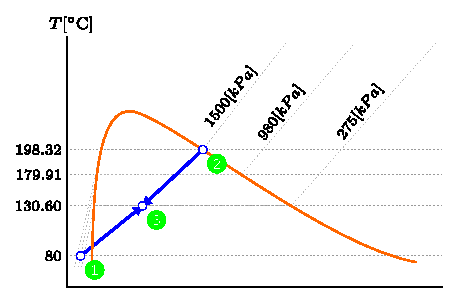
\includegraphics[scale=1.25]{resources/g05_1.eps}
\end{figure}

\ding{175}
\begin{eqnarray*}
    \begin{array}{c}
        P_4 = 200[kPa] \\
        T_4 = -20^\circ C
    \end{array}
    \rightarrow
    \begin{cases}
        X_4 = 0 \\
        h_4 = 173.74[kJ/kg]
    \end{cases}
\end{eqnarray*}

\ding{176}
\begin{eqnarray*}
    \begin{array}{c}
        P_5 = 300[kPa] \\
        T_5 = 50^\circ C
    \end{array}
    \rightarrow
    \begin{cases}
        X_5 > 1 \\
        h_5 = 443.23[kJ/kg]
    \end{cases}
\end{eqnarray*}

\begin{figure}[H]
\centering
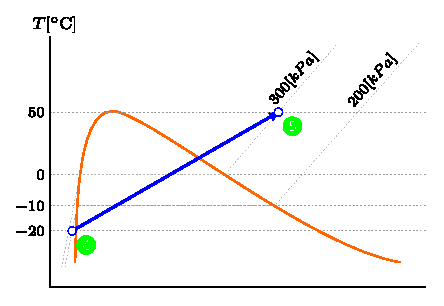
\includegraphics[scale=1.25]{resources/g05_2.eps}
\end{figure}

Se calcula $\dot{m}_4$:

\begin{eqnarray*}
    -\dot{Q} + \dot{m}_1 h_1 + \dot{m}_2 h_2 + \dot{m}_2 \frac{v^2_2}{2}
    + \dot{m}_4 h_4
    = \dot{m}_3 h_3 + \dot{m}_3 \frac{v^2_3}{2} + \dot{m}_4 h_5 \\
    \dot{m}_4 (h_4 - h_5) = \dot{Q} - \dot{m}_1 h_1 - \dot{m}_2 h_2 
    - \dot{m}_2 \frac{v^2_2}{2} + \dot{m}_3 h_3 + \dot{m}_3 \frac{v^2_3}{2}
\end{eqnarray*}

\begin{eqnarray*}
    \frac{v^2_3}{2} &=& \frac{1}{2}\left(100[\frac{m}{min}]\frac{1[min]}{60[s]}\right)^2 \\
                    &=& \frac{1}{2}\frac{100^2}{60^2}[\frac{m^2}{s^2}][\frac{kg}{kg}] \\
                    &=& \frac{25}{18}[\frac{J}{kg}]\frac{1[kJ]}{1000[J]} \\
                    &=& 0.45[\frac{kJ}{kg}]
\end{eqnarray*}

\begin{eqnarray*}
    \frac{v^2_2}{2} &=& \frac{1}{2}\left(165[\frac{m}{min}]\frac{1[min]}{60[s]}\right)^2 \\
                    &=& \frac{1}{2}\frac{165^2}{60^2}[\frac{m^2}{s^2}][\frac{kg}{kg}] \\
                    &=& \frac{121}{32}[\frac{J}{kg}]\frac{1[kJ]}{1000[J]} \\
                    &=& 3.8720[\frac{kJ}{kg}]
\end{eqnarray*}

\begin{eqnarray*}
    \dot{m}_4 &=& \dfrac{\dot{m}_3 h_3 + \dot{m}_3 \dfrac{v^2_3}{2} + \dot{Q} - \dot{m}_1 h_1 - \dot{m}_2 h_2 - \dot{m}_2 \dfrac{v^2_2}{2}}{h_4 - h_5} \\
              &=& \dfrac{\dot{m}_3 h_3 + \dot{m}_3 \dfrac{v^2_3}{2} + \dot{Q}}{h_4 - h_5} - \dfrac{\dot{m}_1 h_1 + \dot{m}_2 h_2 + \dot{m}_2 \dfrac{v^2_2}{2}}{h_4 - h_5} \\
              &=& \dfrac{8663[\frac{kg}{h}]1003.9[\frac{kJ}{kg}] + 8663[\frac{kg}{h}] 0.45[\frac{kJ}{kg}] + 2000[\frac{kJ}{h}]}{173.74[\frac{kJ}{kg}]-443.23[\frac{kJ}{kg}]} \\
              &-& \dfrac{1150[\frac{kg}{h}] 334.88[\frac{kJ}{kg}] + 7513[\frac{kg}{h}] 2792.15[\frac{kJ}{kg}] + 7513[\frac{kg}{h}] 3.8720[\frac{kJ}{kg}]}{173.74[\frac{kJ}{kg}]-443.23[\frac{kJ}{kg}]} \\
              &=& 47085.017[\frac{kg}{h}]
\end{eqnarray*}

\begin{equation*}
\boxed{
    \begin{array}{l}
        \dot{m}_4 = 13.079[\text{kg}/\text{s}]
    \end{array}
}
\end{equation*}

\noindent\rule{15.2cm}{0.4pt}

\item Según la figura se va a acondicionar (enfriar) una casa con 2 equipos de
aire acondicionado (refrigeración). El interior de la casa debe estar a
$18^\circ\text{C}$ y la temperatura exterior es de $30^\circ\text{C}$. El
refrigerador 2 es una maquina de \emph{Carnot}, el 1 tiene un COP de 3, además
el $Q_{EV2} = 2/3 Q_{EV1}$. Si la carga total de enfriamiento es de
$1200[\text{kW}]$. Hallar la potencia total consumida.

\begin{figure}[H]
\centering
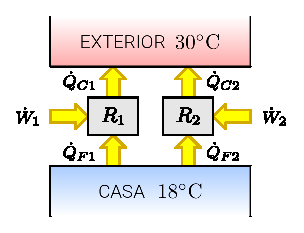
\includegraphics[scale=1.0]{resources/f06.eps}
\end{figure}

\textbf{\underline{Solución}:} \\

\begin{center}
\begin{tabular}{l l}
\ding{172} $R_1$ & \ding{173} $R_2$              \tabularnewline \hline
Maquina Real     & Maquina \emph{Carnot}         \tabularnewline
$T_F=18^\circ C$ & $T_F=18^\circ C$              \tabularnewline
$T_C=30^\circ C$ & $T_C=30^\circ C$              \tabularnewline
$\text{COP}=3$   & $3\dot{Q}_{F2}=2\dot{Q}_{F1}$ \tabularnewline
\end{tabular}
\end{center}

Carga total de enfriamiento: $1200[kW]$.

Se plantean las ecuaciones de equilibrio:

\begin{equation*}
    3\dot{Q}_{F2} = 2\dot{Q}_{F1}
\end{equation*}
\begin{equation*}
    \dot{Q}_{F1} + \dot{Q}_{F2} = 1200[kW]
\end{equation*}

Resolviendo la ecuación lineal se obtiene:

\begin{eqnarray*}
    \dot{Q}_{F1} = 720[kW] \\
    \dot{Q}_{F2} = 480[kW]
\end{eqnarray*}

Se halla el COP para $R_2$:

\begin{equation*}
    \text{COP}_2 = \dfrac{1}{\dfrac{T_C}{T_F} - 1}
          = \dfrac{1}{\dfrac{30+273.15}{18+273.15} - 1}
          = 24.262
\end{equation*}

Se halla el $\dot{W}_2$:

\begin{equation*}
    \text{COP}_2 = \frac{\dot{Q}_{F2}}{\dot{W}_2}
\end{equation*}
\begin{equation*}
    \dot{W}_2 = \frac{\dot{Q}_{F2}}{\text{COP}_2}
              = \frac{480[kW]}{24.262}
              = 19.784[kW]
\end{equation*}

Se halla el $\dot{W}_1$:

\begin{equation*}
    \text{COP}_1 = \frac{\dot{Q}_{F1}}{\dot{W}_1}
\end{equation*}
\begin{equation*}
    \dot{W}_1 = \frac{\dot{Q}_{F1}}{\text{COP}_1}
              = \frac{720[kW]}{3}
              = 240[kW]
\end{equation*}

Se halla la potencia total $\dot{W}_T$:

\begin{equation*}
    \dot{W}_T = \dot{W}_1 + \dot{W}_2
              = 240[kW] + 19.784[kW]
              = 259.78[kW]
\end{equation*}

\begin{equation*}
\boxed{
    \begin{array}{l}
        \dot{W} = 259.78[\text{kW}]
    \end{array}
}
\end{equation*}

\noindent\rule{15.2cm}{0.4pt}

\item Según la figura, se tiene una maquina térmica $[\text{M}_1]$, un equipo de
refrigeración $[\text{R}_1]$ y otro $[\text{R}_2]$. Los equipos $\text{M}_1$ y
$\text{R}_2$ trabajan como maquinas de \emph{Carnot}, en cambio $\text{R}_1$ es
una maquina común el cual tiene un COP de 4. El COP de $\text{R}_2$ es de 3. Si
de todo el trabajo que produce $\text{M}_1$, el $70\%$ entrega a $\text{R}_1$ y
el resto a $\text{R}_2$. Hallar: a) El frío producido por $\text{R}_1$ y
$\text{R}_2$. b) La temperatura $\text{T}_2$.

\begin{figure}[H]
\centering
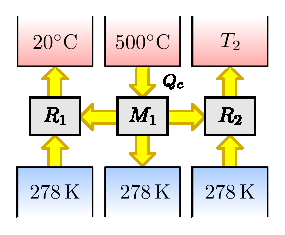
\includegraphics[scale=1.0]{resources/f07.eps}
\end{figure}

\textbf{\underline{Solución}:} \\

\begin{center}
\begin{tabular}{l l l}
\ding{172} $R_1$          & \ding{173} $M_1$      & \ding{174} $R_2$          \tabularnewline \hline
Maquina Real              & Maquina \emph{Carnot} & Maquina \emph{Carnot}     \tabularnewline
$T_F=278 K$               & $T_F=278 K$           & $T_F=278 K$               \tabularnewline
$T_C=20^\circ C$          & $T_C=500^\circ C$     & $T_2=?$                   \tabularnewline
$\text{COP}=4$            & $\dot{Q}_C=1000[kW]$  & $\text{COP}=3$            \tabularnewline
$\dot{W}=0.7\dot{W}_{M1}$ &                       & $\dot{W}=0.3\dot{W}_{M1}$ \tabularnewline
$\dot{Q}_F=?$             &                       & $\dot{Q}_F=?$             \tabularnewline
\end{tabular}
\end{center}

Se halla el rendimiento para $M_1$:

\begin{equation*}
    \eta = 1 - \frac{T_F}{T_C}
         = 1 - \frac{278}{300+273.15}
         = 0.5150
\end{equation*}

Se halla la potencia para $M_1$:

\begin{equation*}
    \eta = \frac{\dot{W}}{\dot{Q}}
\end{equation*}
\begin{equation*}
    \dot{W} = \eta\,\dot{Q}
            = 0.5150(1000[kW])
            = 514.96[kW]
\end{equation*}

Se halla el frío producido para $R_1$:

\begin{equation*}
    \text{COP} = \frac{\dot{Q}}{0.7\dot{W}_{M1}}
\end{equation*}
\begin{equation*}
    \dot{Q} = (\text{COP})(0.7)(\dot{W}_{M1})
            = (4)(0.7)(514.96[kW])
            = 1441.9[kW]
\end{equation*}

Se halla el frío producido para $R_2$:

\begin{equation*}
    \text{COP} = \frac{\dot{Q}}{0.3\dot{W}_{M1}}
\end{equation*}
\begin{equation*}
    \dot{Q} = (\text{COP})(0.3)(\dot{W}_{M1})
            = (3)(0.3)(514.96[kW])
            = 463.47[kW]
\end{equation*}

\begin{equation*}
\boxed{
    \begin{array}{l}
        \dot{Q}_F = 1441.9[\text{kW}] + 463.47[\text{kW}]
                  = 1905.4[\text{kW}]
    \end{array}
}
\end{equation*}

Se halla la temperatura de la fuente caliente para $R_2$:

\begin{equation*}
    \text{COP} = \dfrac{1}{\dfrac{T_C}{T_F} - 1}
\end{equation*}
\begin{equation*}
    \frac{T_C}{T_F} = \frac{1}{\text{COP}} + 1
\end{equation*}
\begin{equation*}
    T_C = T_F\left(\frac{1}{\text{COP}} + 1\right)
        = 278 K\left(\frac{1}{3}+1\right)
        = 370.67 K
\end{equation*}

\begin{equation*}
\boxed{
    \begin{array}{l}
        T_C = 97.52^\circ\text{C}
    \end{array}
}
\end{equation*}

\noindent\rule{15.2cm}{0.4pt}

\item Una maquina térmica de \emph{Carnot} según la figura recibe calor a
$750 K$ y libera calor de desecho al medio ambiente a $27^\circ\text{C}$. Si el
$50\%$ del trabajo total de la maquina térmica se usa para accionar un
refrigerador de \emph{Carnot} que extrae el calor de un espacio refrigerado a
$-15^\circ\text{C}$ a razón de $400[\text{kJ}/\text{min}]$ y lo elimina al medio
ambiente a $27^\circ\text{C}$. Hallar: a) El calor suministrado a la maquina
térmica. b) El calor total liberado al medio ambiente.

\begin{figure}[H]
\centering
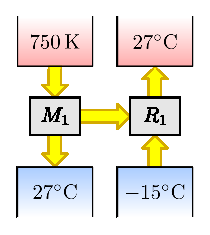
\includegraphics[scale=1.0]{resources/f08.eps}
\end{figure}

\textbf{\underline{Solución}:} \\

\begin{center}
\begin{tabular}{l l}
\ding{172} $M_1$      & \ding{173} $R_1$         \tabularnewline \hline
Maquina \emph{Carnot} & Maquina \emph{Carnot}    \tabularnewline
$T_F=27^\circ C$      & $T_F=-15^\circ C$        \tabularnewline
$T_C=750 K$           & $T_C=27^\circ C$         \tabularnewline
                      & $\dot{W}_R=0.5\dot{W}_M$ \tabularnewline
                      & $Q_F=400[kJ/min]$        \tabularnewline
\end{tabular}
\end{center}

Se halla el COP para $R_1$:

\begin{equation*}
    \text{COP} = \dfrac{1}{\dfrac{T_C}{T_F} - 1}
          = \dfrac{1}{\dfrac{27+273.15}{-15+273.15} - 1}
          = 6.1464
\end{equation*}

Se halla la potencia para $R_1$:

\begin{equation*}
    \text{COP} = \frac{\dot{Q}_F}{\dot{W}}
\end{equation*}
\begin{equation*}
    \dot{W} = \frac{\dot{Q}_F}{\text{COP}}
            = \frac{400[kJ/min]}{6.1464}
            = 65.078[kJ/min]
\end{equation*}

Se halla el rendimiento para $M_1$:

\begin{equation*}
    \eta = 1 - \frac{T_F}{T_C}
         = 1 - \frac{27 + 273.15}{750}
         = 0.5998
\end{equation*}

Se halla el calor suministrado para $M_1$:

\begin{equation*}
    \eta = \frac{\dot{W}}{\dot{Q}}
\end{equation*}
\begin{equation*}
    \dot{Q} = \frac{\dot{W}}{\eta}
            = \frac{2(65.078)}{0.5998}
            = 217.0 [kJ/min]
\end{equation*}

\begin{equation*}
\boxed{
    \begin{array}{l}
        \dot{Q}_C = 217.0[\text{kJ}/\text{min}]
    \end{array}
}
\end{equation*}

Se halla el calor liberado al medio ambiente para $M_1$:

\begin{equation*}
    \dot{Q}_C = \dot{W} + \dot{Q}_F
\end{equation*}
\begin{equation*}
    \dot{Q}_F = \dot{Q}_C - \dot{W}
              = 217.0[kJ/min] - 2(65.078[kJ/min])
              = 86.844[kJ/min]
\end{equation*}

Se halla el calor liberado al medio ambiente para $R_1$:

\begin{equation*}
    \dot{W} + \dot{Q}_F = \dot{Q}_C
\end{equation*}
\begin{equation*}
    \dot{Q}_C = \dot{Q}_F - \dot{W}
              = 400[kJ/min] - 65.078[kJ/min]
              = 465.078[kJ/min]
\end{equation*}

\begin{equation*}
\boxed{
    \begin{array}{l}
        \dot{Q} = 86.844[\text{kJ}/\text{min}] + 465.078[\text{kJ}/\text{min}]
                = 551.92[\text{kJ}/\text{min}]
    \end{array}
}
\end{equation*}

\noindent\rule{15.2cm}{0.4pt}

\item Se emplea R134a en un ciclo ideal de refrigeración ($X_1 = 0$),
($X_3 = 1$) y compresión isoentrópica, que opera entre las temperaturas de
saturación de $-26^\circ\text{C}$ en el evaporador y $40^\circ\text{C}$ en el
condensador. Calcule el frío producido, la potencia del compresor y COP, si el
flujo del refrigerante es $1.2[\text{kg}/\text{s}]$.

\begin{figure}[H]
\centering
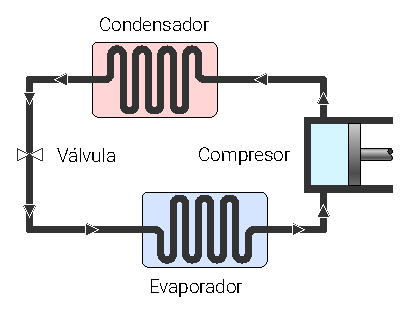
\includegraphics[scale=1.0]{resources/refrigeracion.eps}
\end{figure}

\textbf{\underline{Solución}:} \\

\begin{center}
\begin{tabular}{l l l l}
\ding{172} R134a  & \ding{173} R134a  & \ding{174} R134a  & \ding{175} R134a \tabularnewline \hline
$T_1=40^\circ C$  & $T_2=-26^\circ C$ & $T_3=-26^\circ C$ &                  \tabularnewline
$X_1=0$           &                   & $X_3=1$           &                  \tabularnewline
\end{tabular}
\end{center}

Expansión isoentálpico: $h_1 = h_2$.

Compresión isoentrópica: $s_3 = s_4$.

Flujo de refrigerante: $\dot{m}=1.2[kg/s]$.

\ding{172}
\begin{eqnarray*}
    \begin{array}{c}
        X_1 = 0 \\
        T_1 = 40^\circ C
    \end{array}
    \rightarrow
    \begin{cases}
        P_1 = 1017.0[kPa] \\
        h_1 = 256.54[kJ/kg]
    \end{cases}
\end{eqnarray*}

\ding{173}
\begin{eqnarray*}
    \begin{array}{c}
        T_2 = -26^\circ C
    \end{array}
    \rightarrow
    \begin{cases}
        P_2 = 101.3[kPa] \\
        h_2 = 256.54[kJ/kg]
    \end{cases}
\end{eqnarray*}

\ding{174}
\begin{eqnarray*}
    \begin{array}{c}
        X_3 = 1 \\
        T_3 = -26^\circ C
    \end{array}
    \rightarrow
    \begin{cases}
        P_3 = 101.3[kPa] \\
        h_3 = 382.16[kJ/kg] \\
        s_3 = 1.7453[kJ/kg K]
    \end{cases}
\end{eqnarray*}

\ding{175}
\begin{eqnarray*}
    \begin{array}{c}
        P_4 = 1017.0[kPa] \\
        s_4 = 1.7453[kJ/kg K]
    \end{array}
    \rightarrow
    \begin{cases}
        T_4 = 50^\circ C \\
        h_4 = 431.24[kJ/kg]
    \end{cases}
\end{eqnarray*}

\begin{figure}[H]
\centering
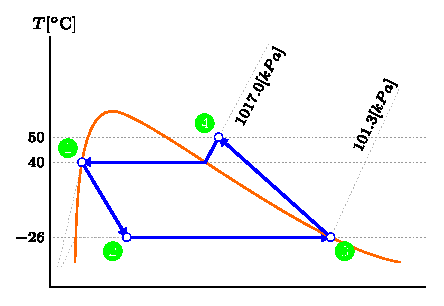
\includegraphics[scale=1.25]{resources/g09.eps}
\end{figure}

Frío producido:

\begin{eqnarray*}
    \dot{Q}_{2\rightarrow3} &=& \dot{m}(h_3 - h_2) \\
                            &=& 1.2[kg/s](382.16[kJ/kg]-256.54[kJ/kg]) \\
                            &=& 150.744[kW]
\end{eqnarray*}

\begin{equation*}
\boxed{
    \begin{array}{l}
        \dot{Q}_{2\rightarrow3} = 150.744[\text{kW}]
    \end{array}
}
\end{equation*}

Potencia del compresor:

\begin{eqnarray*}
    \dot{W}_{3\rightarrow4} &=& \dot{m}(h_4 - h_3) \\
                            &=& 1.2[kg/s](431.24[kJ/kg]-382.16[kJ/kg]) \\
                            &=& 58.896[kW]
\end{eqnarray*}

\begin{equation*}
\boxed{
    \begin{array}{l}
        \dot{W}_{3\rightarrow4} = 58.896[\text{kW}]
    \end{array}
}
\end{equation*}

COP del ciclo:

\begin{eqnarray*}
    \text{COP} &=& \frac{\dot{Q}_{2\rightarrow3}}{\dot{W}_{3\rightarrow4}} \\
               &=& \frac{150.744[kW]}{58.896[kW]} \\
               &=& 2.5595
\end{eqnarray*}

\begin{equation*}
\boxed{
    \begin{array}{l}
        \text{COP} = 2.56
    \end{array}
}
\end{equation*}

\noindent\rule{15.2cm}{0.4pt}

\item El ciclo del problema anterior se usa para un ciclo real con las mismas
presiones, pero con las siguientes modificaciones:
\begin{itemize}
\item El refrigerante sale del evaporador recalentado a $-20^\circ\text{C}$.
\item El refrigerante sale del condensador subenfriado a $30^\circ\text{C}$.
\end{itemize}
Hallar el COP. ¿En cuanto aumenta la producción de frío?

\begin{figure}[H]
\centering
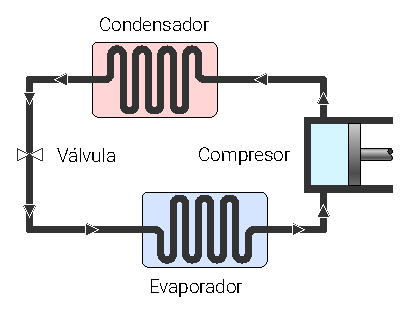
\includegraphics[scale=1.0]{resources/refrigeracion.eps}
\end{figure}

\textbf{\underline{Solución}:} \\

\begin{center}
\begin{tabular}{l l l l}
\ding{172} R134a  & \ding{173} R134a  & \ding{174} R134a  & \ding{175} R134a \tabularnewline \hline
$T_1=30^\circ C$  & $T_2=-26^\circ C$ & $T_3=-20^\circ C$ &                  \tabularnewline
\end{tabular}
\end{center}

Expansión isoentálpica: $h_1 = h_2$.

Compresión isoentrópica: $s_3 = s_4$.

Flujo de refrigerante: $\dot{m}=1.2[kg/s]$.

\ding{172}
\begin{eqnarray*}
    \begin{array}{c}
        T_1 = 30^\circ C
    \end{array}
    \rightarrow
    \begin{cases}
        P_1 = 1017.0[kPa] \\
        h_1 = 241.79[kJ/kg]
    \end{cases}
\end{eqnarray*}

\ding{173}
\begin{eqnarray*}
    \begin{array}{c}
        T_2 = -26^\circ C
    \end{array}
    \rightarrow
    \begin{cases}
        P_2 = 101.3[kPa] \\
        h_2 = 241.79[kJ/kg]
    \end{cases}
\end{eqnarray*}

\ding{174}
\begin{eqnarray*}
    \begin{array}{c}
        T_3 = -20^\circ C
    \end{array}
    \rightarrow
    \begin{cases}
        P_3 = 101.3[kPa] \\
        h_3 = 387.22[kJ/kg] \\
        s_3 = 1.7665[kJ/kg K]
    \end{cases}
\end{eqnarray*}

\ding{175}
\begin{eqnarray*}
    \begin{array}{c}
        P_4 = 1017.0[kPa] \\
        s_4 = 1.7665[kJ/kg K]
    \end{array}
    \rightarrow
    \begin{cases}
        T_4 = 60^\circ C \\
        h_4 = 441.89[kJ/kg]
    \end{cases}
\end{eqnarray*}

\begin{figure}[H]
\centering
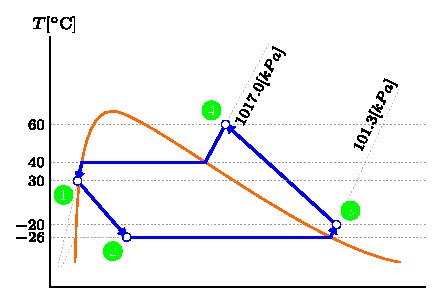
\includegraphics[scale=1.25]{resources/g10.eps}
\end{figure}

Frío producido:

\begin{eqnarray*}
    \dot{Q}_{2\rightarrow3} &=& \dot{m}(h_3 - h_2) \\
                            &=& 1.2[kg/s](387.22[kJ/kg]-241.79[kJ/kg]) \\
                            &=& 174.516[kW]
\end{eqnarray*}

Potencia del compresor:

\begin{eqnarray*}
    \dot{W}_{3\rightarrow4} &=& \dot{m}(h_4 - h_3) \\
                            &=& 1.2[kg/s](441.89[kJ/kg]-387.22[kJ/kg]) \\
                            &=& 65.604[kW]
\end{eqnarray*}

COP del ciclo:

\begin{eqnarray*}
    \text{COP} &=& \frac{\dot{Q}_{2\rightarrow3}}{\dot{W}_{3\rightarrow4}} \\
               &=& \frac{174.516[kW]}{65.604[kW]} \\
               &=& 2.6601
\end{eqnarray*}

\begin{equation*}
\boxed{
    \begin{array}{l}
        \text{COP} = 2.66
    \end{array}
}
\end{equation*}

Incremento en la producción de frío:

\begin{eqnarray*}
    I &=& \frac{\Delta\dot{Q}}{\dot{Q}_9} = \frac{\dot{Q}_{10}-\dot{Q}_9}{\dot{Q}_9} \\
      &=& \frac{174.516[kW]-150.744[kW]}{150.744[kW]} \\
      &=& 0.1577 = 15.77\%
\end{eqnarray*}

\begin{equation*}
\boxed{
    \begin{array}{l}
        \text{Incremento} = 15.77\%
    \end{array}
}
\end{equation*}

\noindent\rule{15.2cm}{0.4pt}

\item En la tabla se tiene los estados de un ciclo de refrigeración que funciona
con R12. El flujo de freón 12 es de $0.05[\text{kg}/\text{s}]$, la potencia de
accionamiento del compresor es de $4[\text{kW}]$. El ciclo se realiza en 2
niveles de presión, y las condiciones operacionales son:

\begin{center}
\begin{tabular}{|c|c|c|c|c|c|c|c|c|}
\hline
& 1 & 2 & 3 & 4 \tabularnewline \hline
$P[\text{kPa}]$ & 320 & 1350 & 1350 & 320 \tabularnewline \hline
$T[^\circ\text{C}]$ & 10 & 120 & 45 & \tabularnewline \hline
\end{tabular}
\end{center}

Hallar: el calor que pierde en el condensador, el calor que absorbe en el
evaporador (frío producido), el COP como ciclo de refrigeración y como bomba de
calor.

\begin{figure}[H]
\centering
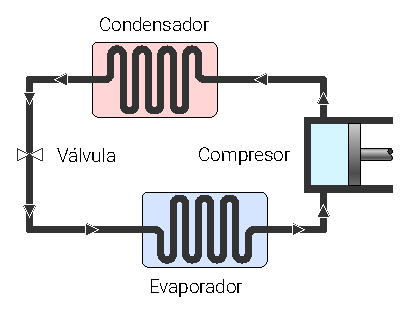
\includegraphics[scale=1.0]{resources/refrigeracion.eps}
\end{figure}

\textbf{\underline{Solución}:} \\

\begin{center}
\begin{tabular}{l l l l}
\ding{172} R-12  & \ding{173} R-12   & \ding{174} R-12  & \ding{175} R-12 \tabularnewline \hline
$T_1=10^\circ C$ & $T_2=120^\circ C$ & $T_3=45^\circ C$ &                 \tabularnewline
$P_1=320[kPa]$   & $P_2=1350[kPa]$   & $P_3=1350[kPa]$  & $P_4=320[kPa]$  \tabularnewline
\end{tabular}
\end{center}

Expansión isoentálpica: $h_1 = h_2$.

Flujo de refrigerante: $\dot{m}=0.05[kg/s]$.

Potencia del compresor: $\dot{W}_{1\rightarrow2}=4[kW]$.

\ding{172}
\begin{eqnarray*}
    \begin{array}{c}
        T_1 = 10^\circ C \\
        P_1 = 320[kPa]
    \end{array}
    \rightarrow
    \begin{cases}
        h_1 = 194.173[kJ/kg]
    \end{cases}
\end{eqnarray*}

\ding{173}
\begin{eqnarray*}
    \begin{array}{c}
        T_2 = 120^\circ C \\
        P_2 = 1350[kPa]
    \end{array}
    \rightarrow
    \begin{cases}
        h_2 = 258.961[kJ/kg]
    \end{cases}
\end{eqnarray*}

\ding{174}
\begin{eqnarray*}
    \begin{array}{c}
        T_3 = 45^\circ C \\
        P_3 = 1350[kPa]
    \end{array}
    \rightarrow
    \begin{cases}
        h_3 = -4.400[kJ/kg]
    \end{cases}
\end{eqnarray*}

\ding{175}
\begin{eqnarray*}
    \begin{array}{c}
        P_4 = 320[kPa]
    \end{array}
    \rightarrow
    \begin{cases}
        T_4 = 0^\circ C \\
        h_4 = -4.400[kJ/kg]
    \end{cases}
\end{eqnarray*}

\begin{figure}[H]
\centering
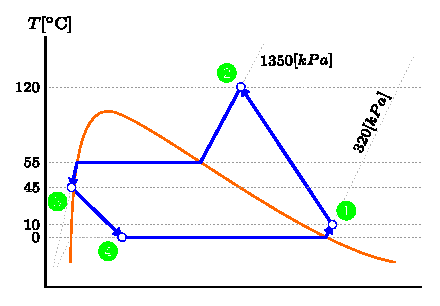
\includegraphics[scale=1.25]{resources/g11.eps}
\end{figure}

Calor que se pierde en el condensador:

\begin{eqnarray*}
    \dot{Q}_{2\rightarrow3} &=& \dot{m}(h_2 - h_3) \\
                            &=& 0.05[kg/s](258.961[kJ/kg]-4.400[kJ/kg]) \\
                            &=& 13.17[kW]
\end{eqnarray*}

\begin{equation*}
\boxed{
    \begin{array}{l}
        \dot{Q}_{2\rightarrow3} = 13.17[\text{kW}]
    \end{array}
}
\end{equation*}

Calor que se absorbe en el evaporador:

\begin{eqnarray*}
    \dot{Q}_{4\rightarrow1} &=& \dot{m}(h_1 - h_4) \\
                            &=& 0.05[kg/s](194.173[kJ/kg]+4.400[kJ/kg]) \\
                            &=& 9.93[kW]
\end{eqnarray*}

\begin{equation*}
\boxed{
    \begin{array}{l}
        \dot{Q}_{4\rightarrow1} = 9.93[\text{kW}]
    \end{array}
}
\end{equation*}

Potencia del compresor:

\begin{eqnarray*}
    \dot{W}_{1\rightarrow2} &=& \dot{m}(h_2 - h_1) \\
                            &=& 0.05[kg/s](258.961[kJ/kg]-194.173[kJ/kg]) \\
                            &=& 3.24[kW]
\end{eqnarray*}

COP del ciclo de refrigeración:

\begin{eqnarray*}
    \text{COP} &=& \frac{\dot{Q}_{4\rightarrow1}}{\dot{W}_{1\rightarrow2}} \\
               &=& \frac{9.93[kW]}{3.24[kW]} \\
               &=& 3.065
\end{eqnarray*}

\begin{equation*}
\boxed{
    \begin{array}{l}
        \text{COP}_{REF} = 3.065
    \end{array}
}
\end{equation*}

COP del ciclo como bomba de calor:

\begin{eqnarray*}
    \text{COP} &=& \frac{\dot{Q}_{2\rightarrow3}}{\dot{W}_{1\rightarrow2}} \\
               &=& \frac{13.17[kW]}{3.24[kW]} \\
               &=& 4.065
\end{eqnarray*}

\begin{equation*}
\boxed{
    \begin{array}{l}
        \text{COP}_{BC} = 4.065
    \end{array}
}
\end{equation*}

\noindent\rule{15.2cm}{0.4pt}

\item En una cámara frigorífica se tiene $10000[\text{kg}]$ de carne de res, el
cual se debe enfriar en 2 horas desde $33^\circ\text{C}$ hasta
$4^\circ\text{C}$, la carne tiene calor especifico de
$0.75[\text{kcal}/\text{kg}\,^\circ\text{C}]$. Dentro la cámara hay 2 personas
que trabaja y liberan calor a razón de $2500[\text{kJ}/\text{h}]$ cada uno. Por
las paredes ingresa flujo de calor a razón de $860[\text{kcal}/\text{h}]$.

Para esta cámara calcular la capacidad de enfriamiento del evaporador. Si el
ciclo de refrigeración trabaja con amoniaco con una temperatura de evaporación
de $-10^\circ\text{C}$ y presión de condensación de $1550[\text{kPa}]$. A la
salida del condensador el refrigerante esta como liquido saturado y tiene un
recalentamiento a la salida del evaporador de $10^\circ\text{C}$. La compresión
en el compresor es isoentrópica. Hallar: el COP de este ciclo de refrigeración,
el flujo de calor que libera por el condensador y el titulo a la salida de la
válvula de expansión.

\begin{figure}[H]
\centering
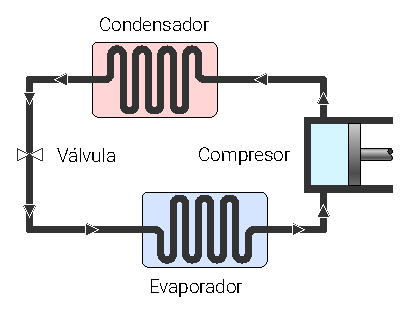
\includegraphics[scale=1.0]{resources/refrigeracion.eps}
\end{figure}

\textbf{\underline{Solución}:} \\

Carne a enfriar:

\begin{equation*}
    m_v = 10000[kg]
\end{equation*}

Tiempo de enfriamiento:

\begin{equation*}
    t_v = 2[h]
\end{equation*}

Temperatura inicial de la carne:
\begin{equation*}
    T_{v0} = 4^\circ C
\end{equation*}

Temperatura final de la carne:
\begin{equation*}
    T_{vf} = 33^\circ C
\end{equation*}

Calor especifico de la carne:
\begin{equation*}
    0.75\left[\dfrac{kcal}{kg ^\circ C}\right]\dfrac{4.1868[kJ]}{1[kcal]}
    = 3.1401\left[\dfrac{kJ}{kg ^\circ C}\right]
\end{equation*}

Flujo de calor requerido para la carne:
\begin{equation*}
    Q_v = m_v\,C_p (T_{vf}-T_{v0})
\end{equation*}
\begin{eqnarray*}
    \dot{Q}_v &=& \frac{m_v}{t_v}\,C_p (T_{vf}-T_{v0}) \\
              &=& \frac{10000[kg]}{2[h]}\,3.1401[\dfrac{kJ}{kg ^\circ C}]\,(33^\circ C-4^\circ C) \\
              &=& 455314.5[kJ/h]
\end{eqnarray*}

Flujo de calor de las personas:
\begin{equation*}
    \dot{Q}_p = 2(2500[kJ/h]) = 5000[kJ/h]
\end{equation*}

Flujo de calor perdido a través de las paredes:
\begin{equation*}
    \dot{Q}_e = 860[\frac{kcal}{h}]\,\frac{4.1868[kJ]}{1[kcal]}
    = 3600.6[kJ/h]
\end{equation*}

Calor total requerido para el enfriamiento:
\begin{eqnarray*}
    \dot{Q}_{EV} &=& \dot{Q}_v + \dot{Q}_p + \dot{Q}_e \\
                 &=& 455314.5[kJ/h] + 5000[kJ/h] + 3600.648[kJ/h] \\
                 &=& 463915.148[kJ/h]
\end{eqnarray*}

\begin{center}
\begin{tabular}{l l l l}
\ding{172} NH-3 & \ding{173} NH-3   & \ding{174} NH-3 & \ding{175} NH-3 \tabularnewline \hline
                & $T_2=-10^\circ C$ & $T_3=0^\circ C$ &                 \tabularnewline
$P_1=1550[kPa]$ &                   &                 & $P_4=1550[kPa]$ \tabularnewline
$X_1=0$         &                   &                 &                 \tabularnewline
\end{tabular}
\end{center}

Compresión isoentrópica: $s_3 = s_4$.

\ding{172}
\begin{eqnarray*}
    \begin{array}{c}
        X_1 = 0 \\
        P_1 = 1550[kPa]
    \end{array}
    \rightarrow
    \begin{cases}
        T_1 = 40^\circ C \\
        h_1 = 371.43[kJ/kg]
    \end{cases}
\end{eqnarray*}

\ding{173}
\begin{eqnarray*}
    \begin{array}{c}
        T_2 = -10^\circ C
    \end{array}
    \rightarrow
    \begin{cases}
        P_2 = 290.9[kPa] \\
        h_2 = 371.43[kJ/kg]
    \end{cases}
\end{eqnarray*}

\ding{174}
\begin{eqnarray*}
    \begin{array}{c}
        T_3 = 0^\circ C
    \end{array}
    \rightarrow
    \begin{cases}
        P_3 = 290.9[kPa] \\
        h_3 = 1454.7[kJ/kg] \\
        s_3 = 5.5420[kJ/kg K]
    \end{cases}
\end{eqnarray*}

\ding{175}
\begin{eqnarray*}
    \begin{array}{c}
        P_4 = 1550[kPa] \\
        s_4 = 5.5420[kJ/kg K]
    \end{array}
    \rightarrow
    \begin{cases}
        T_4 = 120^\circ C \\
        h_4 = 1696.9[kJ/kg]
    \end{cases}
\end{eqnarray*}

\begin{figure}[H]
\centering
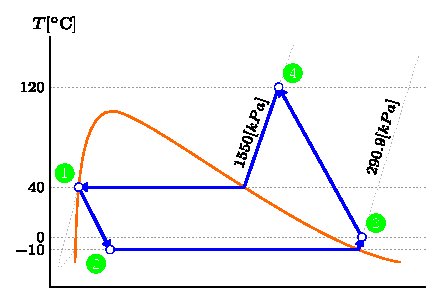
\includegraphics[scale=1.25]{resources/g12.eps}
\end{figure}

Flujo del refrigerante:

\begin{equation*}
    \dot{Q}_{2\rightarrow3} = \dot{m}(h_3 - h_2)
\end{equation*}
\begin{eqnarray*}
    \dot{m} &=& \frac{\dot{Q}_{2\rightarrow3}}{h_3 - h_2} \\
            &=& \frac{463915.148[kJ/h]}{1454.7[kJ/kg]-371.43[kJ/kg]} \\
            &=& 428.25[kg/h]
\end{eqnarray*}

Potencia del compresor:

\begin{eqnarray*}
    \dot{W}_{3\rightarrow4} &=& \dot{m}(h_4 - h_3) \\
                            &=& 428.25[kg/h](1696.9[kJ/kg]-1454.7[kJ/kg]) \\
                            &=& 103723.2166[kJ/h]
\end{eqnarray*}

COP del ciclo de refrigeración:

\begin{eqnarray*}
    \text{COP} &=& \frac{\dot{Q}_{2\rightarrow3}}{\dot{W}_{3\rightarrow4}} \\
               &=& \frac{463915.148[kJ/h]}{103723.2166[kJ/h]} \\
               &=& 4.4726
\end{eqnarray*}

\begin{equation*}
\boxed{
    \begin{array}{l}
        \text{COP}_{REF} = 4.4726
    \end{array}
}
\end{equation*}

Calor que se pierde en el condensador:

\begin{eqnarray*}
    \dot{Q}_{4\rightarrow1} &=& \dot{m}(h_4 - h_1) \\
                            &=& 428.25[kg/h](1696.9[kJ/kg]-371.43[kJ/kg]) \\
                            &=& 567638.3646[kJ/h]
\end{eqnarray*}

\begin{equation*}
\boxed{
    \begin{array}{l}
        \dot{Q}_{4\rightarrow1} = 157.68[kJ/s]
    \end{array}
}
\end{equation*}

Titulo a la salida de la válvula de expansión:

\begin{eqnarray*}
    \begin{array}{c}
        T_2 = -10^\circ C \\
        P_2 = 290.9[kPa] \\
        h_2 = 371.43[kJ/kg]
    \end{array}
    \rightarrow
    \begin{cases}
        h_l = 134.41[kJ/kg] \\
        h_v = 1430.8[kJ/kg]
    \end{cases}
\end{eqnarray*}

\begin{eqnarray*}
    X_2 &=& \frac{h_2 - h_l}{h_v - h_l} \\
        &=& \frac{371.43[kJ/kg]-134.41[kJ/kg]}{1430.8[kJ/kg]-134.41[kJ/kg]} \\
        &=& 0.1828 = 18.28\%
\end{eqnarray*}

\begin{equation*}
\boxed{
    \begin{array}{l}
        X_2 = 18.28\%
    \end{array}
}
\end{equation*}

\noindent\rule{15.2cm}{0.4pt}

\item Una central termoeléctrica según el ciclo de \emph{Rankine}, funciona con
una temperatura de ebullición en el caldero de $150^\circ\text{C}$, una
temperatura de condensación en el condensador de $75^\circ\text{C}$. La
temperatura del vapor a la entrada a la turbina es $400^\circ\text{C}$. El agua
condensada sale del condensador a $40^\circ\text{C}$ para entrar a la bomba de
agua. Los procesos en la bomba y en la turbina son isoentrópicas. La potencia de
la bomba es de $4[\text{kW}]$. Hallar: a) la potencia de la turbina, b) el flujo
de calor en el caldero, c) el calor que libera el agua en el condensador y d) el
rendimiento del ciclo.

\begin{figure}[H]
\centering
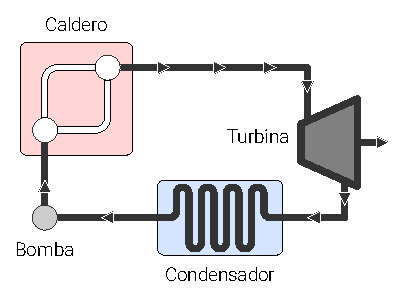
\includegraphics[scale=1.0]{resources/rankine.eps}
\end{figure}

\textbf{\underline{Solución}:} \\

Temperatura de ebullición en el caldero: $150^\circ C$.

Temperatura de condensación en el condensador: $75^\circ C$.

\begin{center}
\begin{tabular}{l l l l}
\ding{172} Agua   & \ding{173} Agua  & \ding{174} Agua  & \ding{175} Agua \tabularnewline \hline
$T_1=400^\circ C$ & & $T_3=40^\circ C$ & \tabularnewline
$P_1=475.9[kPa]$  & $P_2=38.58[kPa]$ & $P_3=38.58[kPa]$ & $P_4=475.9[kPa]$ \tabularnewline
\end{tabular}
\end{center}

Procesos isoentrópicos en la bomba y la turbina:

\begin{eqnarray*}
    s_3 = s_4 \\
    s_1 = s_2
\end{eqnarray*}

Potencia de la bomba: $\dot{Q}_{3\rightarrow4} = 4[kW]$.

\ding{172}
\begin{eqnarray*}
    \begin{array}{c}
        T_1 = 400^\circ C \\
        P_1 = 475.9[kPa]
    \end{array}
    \rightarrow
    \begin{cases}
        h_1 = 3271.83[kJ/kg] \\
        s_1 = 7.7937[kJ/kg K]
    \end{cases}
\end{eqnarray*}

\ding{173}
\begin{eqnarray*}
    \begin{array}{c}
        P_2 = 38.58[kPa] \\
        s_2 = 7.7937[kJ/kg K]
    \end{array}
    \rightarrow
    \begin{cases}
        s_v = 7.6824[kJ/kg K] \\
        T_2 = 100^\circ C \\
        h_2 = 2682.52[kJ/kg]
    \end{cases}
\end{eqnarray*}

\ding{174}
\begin{eqnarray*}
    \begin{array}{c}
        T_3 = 40^\circ C \\
        P_3 = 38.58[kPa]
    \end{array}
    \rightarrow
    \begin{cases}
        h_3 = 167.54[kJ/kg] \\
        s_3 = 0.5724[kJ/kg K] \\
        \nu_3 = 0.001008[m^3/kg]
    \end{cases}
\end{eqnarray*}

\ding{175}
\begin{eqnarray*}
    \begin{array}{c}
        P_4 = 475.9[kPa] \\
        s_4 = 0.5724[kJ/kg K]
    \end{array}
    \rightarrow
    \begin{cases}
        T_4 = 40^\circ C \\
        h_4 = \nu_3 (P_4-P_3) + h_3 = 167.98[kJ/kg]
    \end{cases}
\end{eqnarray*}

\begin{figure}[H]
\centering
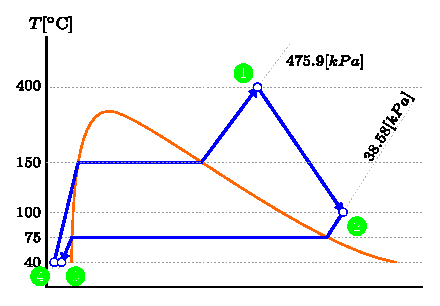
\includegraphics[scale=1.25]{resources/g13.eps}
\end{figure}

Flujo másico de agua:

\begin{equation*}
    \dot{W}_{3\rightarrow4} = \dot{m} (h_4 - h_3)
\end{equation*}
\begin{eqnarray*}
    \dot{m} &=& \frac{\dot{W}_{3\rightarrow4}}{h_3 - h_4} \\
            &=& \frac{4[kW]}{167.98[kJ/kg]-167.54[kJ/kg]} \\
            &=& 9.0740[kg/s]
\end{eqnarray*}

Potencia de la turbina:

\begin{eqnarray*}
    \dot{W}_{1\rightarrow2} &=& \dot{m}(h_1 - h_2) \\
                            &=& 9.0740[kg/s](3271.83[kJ/kg]-2682.52[kJ/kg]) \\
                            &=& 5347.4[kW]
\end{eqnarray*}

\begin{equation*}
\boxed{
    \begin{array}{l}
        \dot{W}_{1\rightarrow2} = 5347.4[kW]
    \end{array}
}
\end{equation*}

Flujo de calor en el caldero:

\begin{eqnarray*}
    \dot{Q}_{4\rightarrow1} &=& \dot{m}(h_1 - h_4) \\
                            &=& 9.0740[kg/s](3271.83[kJ/kg]-167.98[kJ/kg]) \\
                            &=& 28164.4147[kW]
\end{eqnarray*}

\begin{equation*}
\boxed{
    \begin{array}{l}
        \dot{Q}_{4\rightarrow1} = 28164.41[kW]
    \end{array}
}
\end{equation*}

Calor que libera el agua en el condensador:

\begin{eqnarray*}
    \dot{Q}_{2\rightarrow3} &=& \dot{m}(h_2 - h_3) \\
                            &=& 9.0740[kg/s](2682.52[kJ/kg]-167.54[kJ/kg]) \\
                            &=& 22820.9992[kW]
\end{eqnarray*}

\begin{equation*}
\boxed{
    \begin{array}{l}
        \dot{Q}_{2\rightarrow3} = 22821[kW]
    \end{array}
}
\end{equation*}

Rendimiento del ciclo:

\begin{eqnarray*}
    \eta &=& \frac{\dot{W}_{1\rightarrow2}}
             {\dot{W}_{3\rightarrow4}+\dot{Q}_{4\rightarrow1}} \\
         &=& \frac{5347.5[kW]}{4[kW]+28164.41[kW]} \\
         &=& 0.1898 = 18.98\%
\end{eqnarray*}

\begin{equation*}
\boxed{
    \begin{array}{l}
        \eta = 18.98\%
    \end{array}
}
\end{equation*}

\noindent\rule{15.2cm}{0.4pt}

\item Se tiene un ciclo de \emph{Rankine} que funciona entre las presiones de
$4[\text{MPa}]$ y $0,4[\text{kg}/\text{cm}^2]$. El vapor sale e ingresa a la
turbina a $400^\circ\text{C}$. El condensado sale del condensador a
$40^\circ\text{C}$ para entrar a la bomba de agua. Los procesos en la bomba y en
la turbina son reversibles. Si el flujo de agua es de $1[\text{kg}/\text{s}]$.

Hallar: a) la potencia de la turbina, b) el flujo de calor en el caldero, c) el
calor que libera el agua en el condensador, d) el rendimiento del ciclo, e) si
el ciclo fuera teórico hallar su rendimiento, f) cual de los ciclos tiene mayor
rendimiento, g) ¿a que se debe la diferencia?

\begin{figure}[H]
\centering
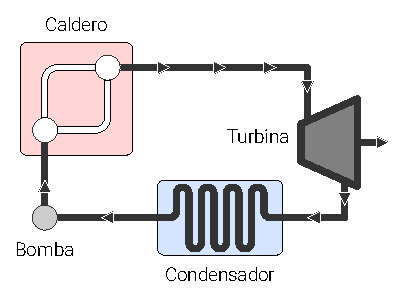
\includegraphics[scale=1.0]{resources/rankine.eps}
\end{figure}

\textbf{\underline{Solución}:} \\

Presión en el caldero: $P_1 = 4000[kPa]$.

Presión en el condensador:

\begin{equation*}
    P_2 = 0.4\left[\frac{kgf}{cm^2}\right]\frac{980[N]}{1[kgf]}
          \frac{100[cm]}{1[m]}\frac{100[cm]}{1[m]}\frac{1[kPa]}{1[Pa]}
        = 39.2[kPa]
\end{equation*}

\begin{center}
\begin{tabular}{l l l l}
\ding{172} Agua   & \ding{173} Agua   & \ding{174} Agua  & \ding{175} Agua \tabularnewline \hline
$T_1=400^\circ C$ &                   & $T_3=40^\circ C$ &                 \tabularnewline
$P_1=4000[kPa]$   & $P_2=39.2[kPa]$   & $P_3=39.2[kPa]$  & $P_4=4000[kPa]$ \tabularnewline
\end{tabular}
\end{center}

Procesos reversibles en la bomba y la turbina:

\begin{eqnarray*}
    s_1 = s_2 \\
    s_3 = s_4
\end{eqnarray*}

Flujo de agua: $1[kg/s]$.

\ding{172}
\begin{eqnarray*}
    \begin{array}{c}
        T_1 = 400^\circ C \\
        P_1 = 4000[kPa]
    \end{array}
    \rightarrow
    \begin{cases}
        h_1 = 3213.51[kJ/kg] \\
        s_1 = 6.7689[kJ/kg K]
    \end{cases}
\end{eqnarray*}

\ding{173}
\begin{eqnarray*}
    \begin{array}{c}
        P_2 = 39.2[kPa] \\
        s_2 = 6.7689[kJ/kg K]
    \end{array}
    \rightarrow
    \begin{cases}
        s_l = 1.0258[kJ/kg K] \\
        s_v = 7.6700[kJ/kg K] \\
        X_2 = \dfrac{s_2 - s_l}{s_v - s_l} = 0.8644 \\
        h_l = 317.55[kJ/kg] \\
        h_v = 2636.74[kJ/kg] \\
        h_2 = h_l + X_2 (h_v - h_l) = 2322.2[kJ/kg]
    \end{cases}
\end{eqnarray*}

\ding{174}
\begin{eqnarray*}
    \begin{array}{c}
        T_3 = 40^\circ C \\
        P_3 = 39.2[kPa]
    \end{array}
    \rightarrow
    \begin{cases}
        h_3 = 167.54[kJ/kg] \\
        s_3 = 0.5724[kJ/kg K] \\
        \nu_3 = 0.001008[m^3/kg]
    \end{cases}
\end{eqnarray*}

\ding{175}
\begin{eqnarray*}
    \begin{array}{c}
        P_4 = 4000[kPa] \\
        s_4 = 0.5724[kJ/kg K]
    \end{array}
    \rightarrow
    \begin{cases}
        T_4 = 40^\circ C \\
        h_4 = \nu_3 (P_4 - P_3) + h_3 = 171.53[kJ/kg]
    \end{cases}
\end{eqnarray*}

\begin{figure}[H]
\centering
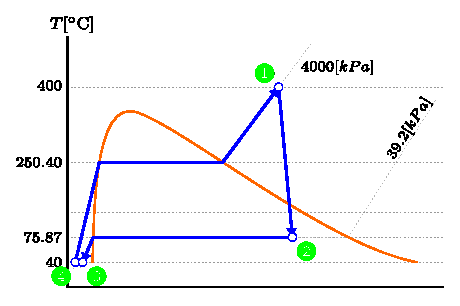
\includegraphics[scale=1.25]{resources/g14_1.eps}
\end{figure}

Potencia de la turbina:

\begin{eqnarray*}
    \dot{W}_{1\rightarrow2} &=& \dot{m}(h_1 - h_2) \\
                            &=& 1[kg/s](3213.5[kJ/kg]-2322.2[kJ/kg]) \\
                            &=& 891.30[kW]
\end{eqnarray*}

\begin{equation*}
\boxed{
    \begin{array}{l}
        \dot{W}_{1\rightarrow2} = 891.30[kW]
    \end{array}
}
\end{equation*}

Flujo de calor en el caldero:

\begin{eqnarray*}
    \dot{Q}_{4\rightarrow1} &=& \dot{m}(h_1 - h_4) \\
                            &=& 1[kg/s](3213.5[kJ/kg]-171.53[kJ/kg]) \\
                            &=& 3042.0[kW]
\end{eqnarray*}

\begin{equation*}
\boxed{
    \begin{array}{l}
        \dot{Q}_{4\rightarrow1} = 3042.0[kW]
    \end{array}
}
\end{equation*}

Calor que libera el agua en el condensador:

\begin{eqnarray*}
    \dot{Q}_{2\rightarrow3} &=& \dot{m}(h_2 - h_3) \\
                            &=& 1[kg/s](2322.2[kJ/kg]-167.54[kJ/kg]) \\
                            &=& 2154.7[kW]
\end{eqnarray*}

\begin{equation*}
\boxed{
    \begin{array}{l}
        \dot{Q}_{2\rightarrow3} = 2154.7[kW]
    \end{array}
}
\end{equation*}

Potencia de la bomba:

\begin{eqnarray*}
    \dot{W}_{3\rightarrow4} &=& \dot{m}(h_4 - h_3) \\
                            &=& 1[kg/s](171.53[kJ/kg]-167.54[kJ/kg]) \\
                            &=& 3.9925[kW]
\end{eqnarray*}

Rendimiento del ciclo:

\begin{eqnarray*}
    \eta &=& \frac{\dot{W}_{1\rightarrow2}}
             {\dot{W}_{3\rightarrow4}+\dot{Q}_{4\rightarrow1}} \\
         &=& \frac{891.30[kW]}{3.9925[kW]+3042.0[kW]} \\
         &=& 0.2926 = 29.26\%
\end{eqnarray*}

\begin{equation*}
\boxed{
    \begin{array}{l}
        \eta = 29.26\%
    \end{array}
}
\end{equation*}

Considerando un ciclo teórico: $X_2 = 1$

\begin{figure}[H]
\centering
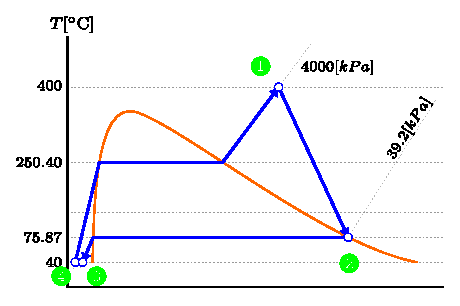
\includegraphics[scale=1.25]{resources/g14_2.eps}
\end{figure}

\ding{173}
\begin{eqnarray*}
    \begin{array}{c}
        P_2 = 39.2[kPa] \\
        X_2 = 1
    \end{array}
    \rightarrow
    \begin{cases}
        h_2 = 2636.74[kJ/kg]
    \end{cases}
\end{eqnarray*}

Potencia de la turbina:

\begin{eqnarray*}
    \dot{W}_{1\rightarrow2} &=& \dot{m}(h_1 - h_2) \\
                            &=& 1[kg/s](3213.5[kJ/kg]-2636.7[kJ/kg]) \\
                            &=& 576.77[kW]
\end{eqnarray*}

Rendimiento del ciclo:

\begin{eqnarray*}
    \eta &=& \frac{\dot{W}_{1\rightarrow2}}
             {\dot{W}_{3\rightarrow4}+\dot{Q}_{4\rightarrow1}} \\
         &=& \frac{576.77[kW]}{3.9925[kW]+3042.0[kW]} \\
         &=& 0.1894 = 18.94\%
\end{eqnarray*}

\begin{equation*}
\boxed{
    \begin{array}{l}
        \eta = 18.94\%
    \end{array}
}
\end{equation*}

El rendimiento del primer ciclo es mayor: $29.26\% > 18.94\%$.

Esta diferencia se debe a la cantidad de potencia generada en el segundo caso:
$891.30[kW] > 576.77[kW]$.

\noindent\rule{15.2cm}{0.4pt}

\item Una planta termoeléctrica (ciclo de \emph{Rankine}) funciona entre las
presiones de $10[\text{kPa}]$ y $2[\text{MPa}]$ con una temperatura máxima de
$400^\circ\text{C}$ a la salida del caldero. El agua a la entrada a la bomba
esta como liquido saturado. Si la expansión en la turbina es isoentrópica, la
potencia de la bomba es de $2[\text{kJ}/\text{kg}]$ y el flujo másico de
$2[\text{kg}/\text{s}]$. Hallar la potencia generada en la turbina, el calor
liberado por el condensador y el rendimiento del ciclo.

\begin{figure}[H]
\centering
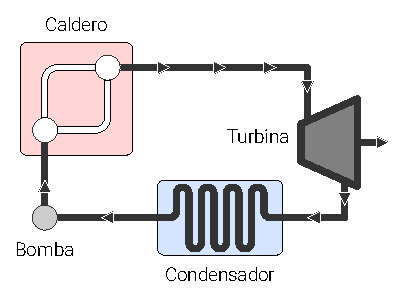
\includegraphics[scale=1.0]{resources/rankine.eps}
\end{figure}

\textbf{\underline{Solución}:} \\

Presión en el caldero: $P_1 = 2000[kPa]$.

Presión en el condensador: $P_3 = 10[kPa]$.

\begin{center}
\begin{tabular}{l l l l}
\ding{172} Agua   & \ding{173} Agua & \ding{174} Agua & \ding{175} Agua \tabularnewline \hline
$T_1=400^\circ C$ &                 &                 &                 \tabularnewline
$P_1=2000[kPa]$   & $P_2=10[kPa]$   & $P_3=10[kPa]$   & $P_4=2000[kPa]$ \tabularnewline
                  &                 & $X_3=0$         &                 \tabularnewline
\end{tabular}
\end{center}

Proceso isoentrópico en la turbina: $s_1 = s_2$.

Potencia de la bomba: $h_4 - h_3 = 2[kJ/kg]$.

Flujo másico: $2[kg/s]$.

\ding{172}
\begin{eqnarray*}
    \begin{array}{c}
        T_1 = 400^\circ C \\
        P_1 = 2000[kPa]
    \end{array}
    \rightarrow
    \begin{cases}
        h_1 = 3247.60[kJ/kg] \\
        s_1 = 7.1270[kJ/kg K]
    \end{cases}
\end{eqnarray*}

\ding{173}
\begin{eqnarray*}
    \begin{array}{c}
        P_2 = 10[kPa] \\
        s_2 = 7.1270[kJ/kg K]
    \end{array}
    \rightarrow
    \begin{cases}
        s_l = 0.6492[kJ/kg K] \\
        s_v = 8.1501[kJ/kg K] \\
        X_2 = \dfrac{s_2 - s_l}{s_v - s_l} = 0.8636 \\
        h_l = 191.81[kJ/kg] \\
        h_v = 2584.63[kJ/kg] \\
        h_2 = h_l + X_2 (h_v - h_l) = 2258.3[kJ/kg]
    \end{cases}
\end{eqnarray*}

\ding{174}
\begin{eqnarray*}
    \begin{array}{c}
        P_3 = 10[kPa] \\
        X_3 = 0
    \end{array}
    \rightarrow
    \begin{cases}
        h_3 = 191.81[kJ/kg]
    \end{cases}
\end{eqnarray*}

\ding{175}
\begin{eqnarray*}
    \begin{array}{c}
        P_4 = 2000[kPa]
    \end{array}
    \rightarrow
    \begin{cases}
        h_4 = 2[kJ/kg] + h_3 = 193.81[kJ/kg]
    \end{cases}
\end{eqnarray*}

\begin{figure}[H]
\centering
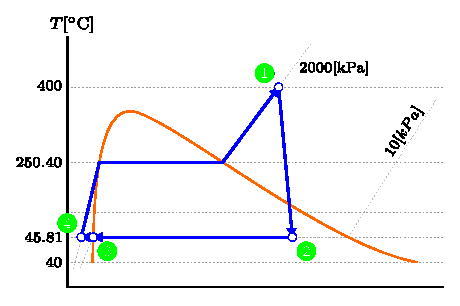
\includegraphics[scale=1.25]{resources/g15.eps}
\end{figure}

Potencia de la turbina:

\begin{eqnarray*}
    \dot{W}_{1\rightarrow2} &=& \dot{m}(h_1 - h_2) \\
                            &=& 2[kg/s](3247.6[kJ/kg]-2258.3[kJ/kg]) \\
                            &=& 1978.7[kW]
\end{eqnarray*}

\begin{equation*}
\boxed{
    \begin{array}{l}
        \dot{W}_{1\rightarrow2} = 1978.7[kW]
    \end{array}
}
\end{equation*}

Calor que libera el condensador:

\begin{eqnarray*}
    \dot{Q}_{2\rightarrow3} &=& \dot{m}(h_2 - h_3) \\
                            &=& 2[kg/s](2258.3[kJ/kg]-191.81[kJ/kg]) \\
                            &=& 4132.9[kW]
\end{eqnarray*}

\begin{equation*}
\boxed{
    \begin{array}{l}
        \dot{Q}_{2\rightarrow3} = 4132.9[kW]
    \end{array}
}
\end{equation*}

Potencia de la bomba:

\begin{eqnarray*}
    \dot{W}_{3\rightarrow4} &=& \dot{m}(h_4 - h_3) \\
                            &=& 2[kg/s](193.81[kJ/kg]-191.81[kJ/kg]) \\
                            &=& 4[kW]
\end{eqnarray*}

Flujo de calor en el caldero:

\begin{eqnarray*}
    \dot{Q}_{4\rightarrow1} &=& \dot{m}(h_1 - h_4) \\
                            &=& 2[kg/s](3247.6[kJ/kg]-193.81[kJ/kg]) \\
                            &=& 6107.6[kW]
\end{eqnarray*}

Rendimiento del ciclo:

\begin{eqnarray*}
    \eta &=& \frac{\dot{W}_{1\rightarrow2}}
             {\dot{W}_{3\rightarrow4}+\dot{Q}_{4\rightarrow1}} \\
         &=& \frac{1978.7[kW]}{4[kW]+6107.6[kW]} \\
         &=& 0.3238 = 32.38\%
\end{eqnarray*}

\begin{equation*}
\boxed{
    \begin{array}{l}
        \eta = 32.38\%
    \end{array}
}
\end{equation*}

\noindent\rule{15.2cm}{0.4pt}

\item Si se aumenta la presión en la caldera a $4[\text{MPa}]$ en el problema
anterior y la potencia de la bomba sube a $3[\text{kJ}/\text{kg}]$,
manteniéndose todas las otras condiciones. Hallar la eficiencia del ciclo. ¿Esta
eficiencia bajó o aumentó?, ¿Por qué?

\begin{figure}[H]
\centering
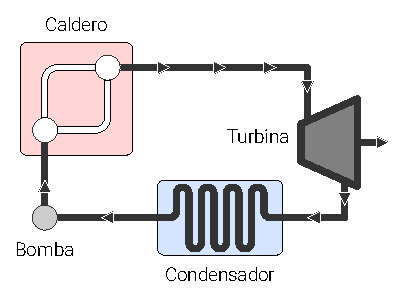
\includegraphics[scale=1.0]{resources/rankine.eps}
\end{figure}

\textbf{\underline{Solución}:} \\

Presión en el caldero: $P_1 = 4000[kPa]$.

Presión en el condensador: $P_3 = 10[kPa]$.

\begin{center}
\begin{tabular}{l l l l}
\ding{172} Agua   & \ding{173} Agua & \ding{174} Agua & \ding{175} Agua \tabularnewline \hline
$T_1=400^\circ C$ &                 &                 &                 \tabularnewline
$P_1=4000[kPa]$   & $P_2=10[kPa]$   & $P_3=10[kPa]$   & $P_4=4000[kPa]$ \tabularnewline
                  &                 & $X_3=0$         &                 \tabularnewline
\end{tabular}
\end{center}

Proceso isoentrópico en la turbina: $s_1 = s_2$.

Potencia de la bomba: $h_4 - h_3 = 3[kJ/kg]$.

Flujo másico: $2[kg/s]$.

\ding{172}
\begin{eqnarray*}
    \begin{array}{c}
        T_1 = 400^\circ C \\
        P_1 = 4000[kPa]
    \end{array}
    \rightarrow
    \begin{cases}
        h_1 = 3213.51[kJ/kg] \\
        s_1 = 6.7689[kJ/kg K]
    \end{cases}
\end{eqnarray*}

\ding{173}
\begin{eqnarray*}
    \begin{array}{c}
        P_2 = 10[kPa] \\
        s_2 = 6.7689[kJ/kg K]
    \end{array}
    \rightarrow
    \begin{cases}
        s_l = 0.6492[kJ/kg K] \\
        s_v = 8.1501[kJ/kg K] \\
        X_2 = \dfrac{s_2 - s_l}{s_v - s_l} = 0.8159 \\
        h_l = 191.81[kJ/kg] \\
        h_v = 2584.63[kJ/kg] \\
        h_2 = h_l + X_2 (h_v - h_l) = 2144.0[kJ/kg]
    \end{cases}
\end{eqnarray*}

\ding{174}
\begin{eqnarray*}
    \begin{array}{c}
        P_3 = 10[kPa] \\
        X_3 = 0
    \end{array}
    \rightarrow
    \begin{cases}
        h_3 = 191.81[kJ/kg]
    \end{cases}
\end{eqnarray*}

\ding{175}
\begin{eqnarray*}
    \begin{array}{c}
        P_4 = 4000[kPa]
    \end{array}
    \rightarrow
    \begin{cases}
        h_4 = 3[kJ/kg] + h_3 = 194.81[kJ/kg]
    \end{cases}
\end{eqnarray*}

\begin{figure}[H]
\centering
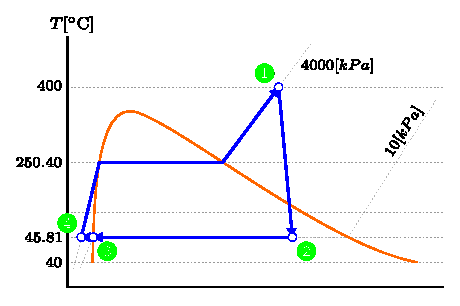
\includegraphics[scale=1.25]{resources/g16.eps}
\end{figure}

Potencia de la turbina:

\begin{eqnarray*}
    \dot{W}_{1\rightarrow2} &=& \dot{m}(h_1 - h_2) \\
                            &=& 2[kg/s](3213.5[kJ/kg]-2144.0[kJ/kg]) \\
                            &=& 2139.0[kW]
\end{eqnarray*}

Potencia de la bomba:

\begin{eqnarray*}
    \dot{W}_{3\rightarrow4} &=& \dot{m}(h_4 - h_3) \\
                            &=& 2[kg/s](194.81[kJ/kg]-191.81[kJ/kg]) \\
                            &=& 6[kW]
\end{eqnarray*}

Flujo de calor en el caldero:

\begin{eqnarray*}
    \dot{Q}_{4\rightarrow1} &=& \dot{m}(h_1 - h_4) \\
                            &=& 2[kg/s](3213.5[kJ/kg]-194.81[kJ/kg]) \\
                            &=& 6037.4[kW]
\end{eqnarray*}

Rendimiento del ciclo:

\begin{eqnarray*}
    \eta &=& \frac{\dot{W}_{1\rightarrow2}}
             {\dot{W}_{3\rightarrow4}+\dot{Q}_{4\rightarrow1}} \\
         &=& \frac{2139[kW]}{6[kW]+6037.4[kW]} \\
         &=& 0.3539 = 35.39\%
\end{eqnarray*}

\begin{equation*}
\boxed{
    \begin{array}{l}
        \eta = 35.39\%
    \end{array}
}
\end{equation*}

Comparación entre ambos casos:

\begin{center}
\begin{tabular}{l|c c}
                          & Caso \ding{172} & Caso \ding{173} \tabularnewline \hline
$\dot{W}_{1\rightarrow2}$ & $1978.7[kW]$    & $2139.0[kW]$    \tabularnewline
$\dot{W}_{3\rightarrow4}$ & $4[kW]$         & $6[kW]$         \tabularnewline
$\dot{Q}_{4\rightarrow1}$ & $6107.6[kW]$    & $6037.4[kW]$    \tabularnewline
$\eta$                    & $32.38\%$       & $35.39\%$       \tabularnewline
\end{tabular}
\end{center}

El segundo caso tiene mayor eficiencia al generar mas potencia en la turbina
$1978.7[kW] < 2139.0[kW]$ con un menor calor en el caldero
$6107.6[kW] > 6037.4[kW]$.

\noindent\rule{15.2cm}{0.4pt}

\end{enumerate}

\end{document}

